\documentclass[conference]{IEEEtran}
\IEEEoverridecommandlockouts

\usepackage[spanish]{babel}
\usepackage[utf8]{inputenc}
\usepackage[T1]{fontenc}
\usepackage{cite}
\usepackage{amsmath,amssymb,amsfonts}
\usepackage{graphicx}
\usepackage{textcomp}
\usepackage{xcolor}
\usepackage{booktabs}
\usepackage{algorithm}
\usepackage{algpseudocode}
\usepackage{listings}
\usepackage{tikz}
\usetikzlibrary{shapes.geometric,arrows.meta,positioning,fit,backgrounds,calc,decorations.pathreplacing,babel}

\lstset{
  basicstyle=\ttfamily\scriptsize,
  backgroundcolor=\color{gray!10},
  frame=single,
  breaklines=true,
  showstringspaces=false,
  columns=flexible,
}

% Spanish algorithm keywords
\algrenewcommand\algorithmicfor{\textbf{para cada}}
\algrenewcommand\algorithmicdo{\textbf{hacer}}
\algrenewcommand\algorithmicif{\textbf{si}}
\algrenewcommand\algorithmicthen{\textbf{entonces}}
\algrenewcommand\algorithmicelse{\textbf{si no}}
\algrenewcommand\algorithmicend{\textbf{fin}}
\algrenewcommand\algorithmicreturn{\textbf{retornar}}
\algrenewcommand\algorithmicensure{\textbf{Garantiza:}}
\algrenewcommand\algorithmicrequire{\textbf{Requiere:}}
\algrenewcommand\algorithmicwhile{\textbf{mientras}}

\begin{document}

\title{Dise\~no e Implementaci\'on: Videojuego Shooter Multijugador en Red\\
{\footnotesize Proyecto \#2 --- IC-7602 Redes --- Segunda Etapa --- Grupo 1}}

\author{
\IEEEauthorblockN{Ignacio Brenes M\'endez, Estefan\'ia Delgado Castillo,
Javier D\'iaz Jim\'enez, Mariano Mayorga Halabi, Andrey Ure\~na Berm\'udez}
\IEEEauthorblockA{\textit{Escuela de Ingenier\'ia en Computaci\'on}\\
Instituto Tecnol\'ogico de Costa Rica, Cartago, Costa Rica\\
I Semestre 2026 --- Profesor: Ing. Eduardo A. Canessa Montero, M.Sc.}
}

\maketitle

\begin{abstract}
Este documento presenta el dise\~no modular y la implementaci\'on del videojuego tipo \textit{shooter} multijugador en red para hasta cuatro jugadores simult\'aneos. Se describe la arquitectura cliente-servidor autoritativa con comunicaci\'on UDP, los diagramas de bloques en tres niveles, la implementaci\'on de cada m\'odulo funcional y las pruebas de verificaci\'on realizadas. El sistema fue desarrollado en Python 3.13 utilizando Pygame para el renderizado e incluye predicci\'on local de movimiento, sistema de \textit{pickups}, armas semi-autom\'aticas, colisiones con obst\'aculos, sistema de fases con \textit{ready check} y ranking final.
\end{abstract}

%=============================================================
\section{Dise\~no Modular}
%=============================================================

\subsection{Arquitectura General del Sistema --- Nivel 1}

La Fig.~\ref{fig:arq} muestra la vista de primer nivel: tres bloques funcionales principales (Cliente, Servidor y M\'odulos Comunes) comunicados mediante el protocolo UDP~\cite{rfc768,forouzan2012}.

\begin{figure}[!h]
    \centering
    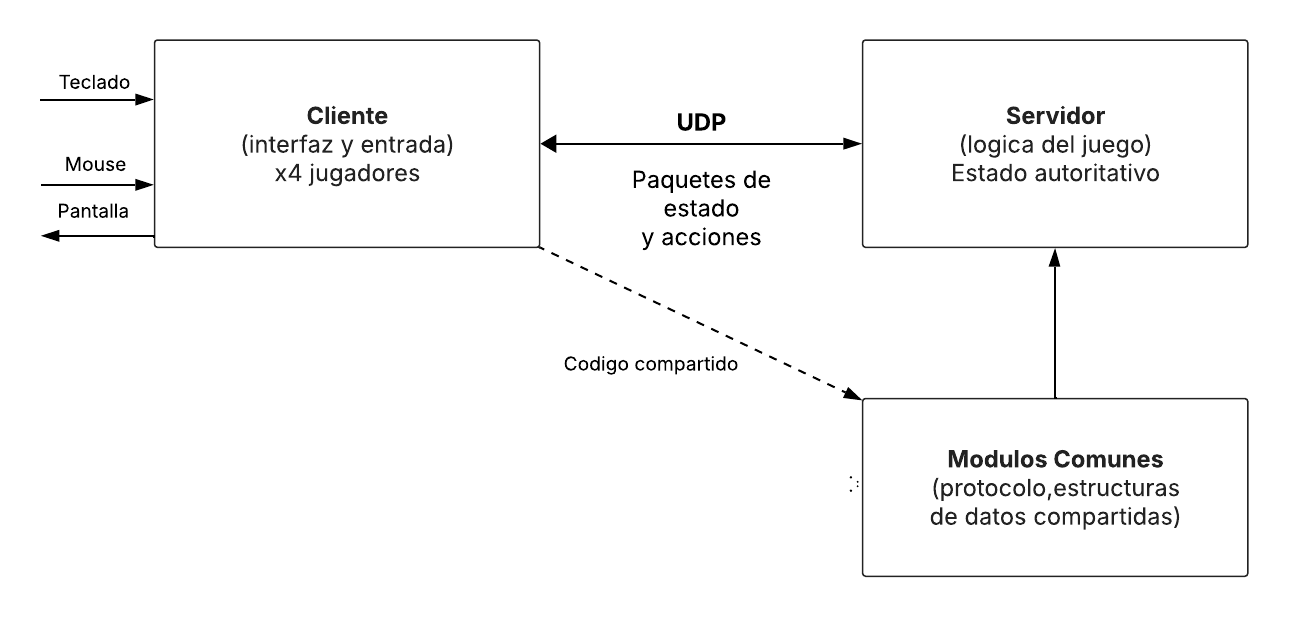
\includegraphics[width=0.95\columnwidth]{Imagenes/arq.png}
    \caption{Diagrama de Arquitectura General.}
    \label{fig:arq}
\end{figure}

\textbf{Cliente (interfaz y entrada):} Captura eventos de teclado (movimiento WASD/flechas) y mouse (apuntado y disparo), los serializa como paquetes UDP y renderiza el estado recibido. Utiliza tres hilos independientes: hilo principal (eventos + renderizado), hilo de env\'io (30~Hz) e hilo de recepci\'on. Soporta hasta cuatro instancias simult\'aneas.

\textbf{Servidor (l\'ogica del juego):} Autoridad central que mantiene posiciones de jugadores, proyectiles activos, colisiones con obst\'aculos, \textit{pickups}, puntajes, fases de la partida y temporizador. Toda la l\'ogica de juego se ejecuta exclusivamente en el servidor~\cite{gambetta2018}.

\textbf{Comunicaci\'on UDP~\cite{rfc768}:} Se prefiere UDP sobre TCP porque en tiempo real la baja latencia supera la importancia de la entrega garantizada~\cite{tanenbaum2011}. El flujo es bidireccional: los clientes env\'ian acciones a 30~Hz y el servidor difunde el estado actualizado a 20~Hz.

\textbf{M\'odulos Comunes (\texttt{common.py}):} C\'odigo compartido que define constantes f\'isicas (velocidades, radios, cooldowns), funciones de utilidad matem\'atica (\texttt{normalize}, \texttt{clamp}, \texttt{distance\_squared}), funciones de colisi\'on (\texttt{circle\_rect\_overlap}, \texttt{push\_circle\_from\_rect}), serializaci\'on/deserializaci\'on JSON, y generaci\'on determin\'istica de obst\'aculos.

\subsection{Diagrama de Caja Negra}

La Fig.~\ref{fig:cajaNegra} presenta el sistema como caja negra, identificando entradas, salidas y restricciones.

\begin{figure}[!h]
    \centering
    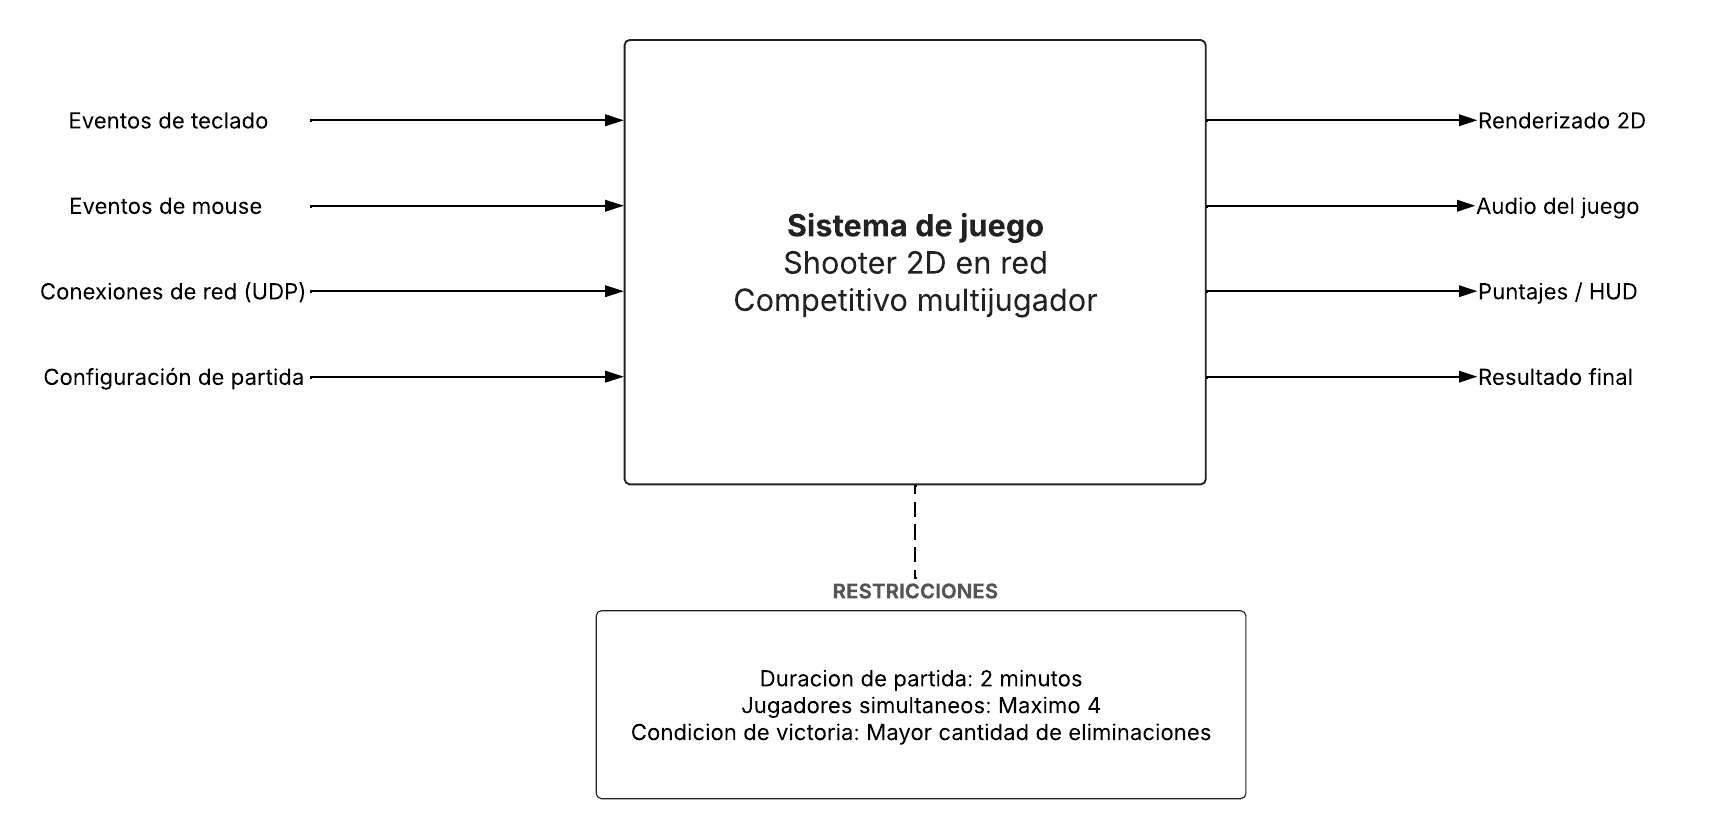
\includegraphics[width=0.95\columnwidth]{Imagenes/cajaNegra.png}
    \caption{Diagrama de Caja Negra.}
    \label{fig:cajaNegra}
\end{figure}

\textbf{Entradas:} (i)~Eventos de teclado WASD/flechas; (ii)~Posici\'on del mouse y clic izquierdo; (iii)~Conexiones UDP con nombre del jugador; (iv)~Mensaje de \textit{ready} para iniciar partida.

\textbf{Salidas:} (i)~Renderizado 2D con mapa militar, tanques, proyectiles, obst\'aculos y pickups; (ii)~Audio: disparos, impactos, eliminaciones y fin de partida; (iii)~HUD con timer, HP, kills, indicador de arma potenciada; (iv)~Pantalla de ranking con kills, muertes y da\~no.

\textbf{Restricciones:} M\'aximo 4 jugadores; victoria por 3 eliminaciones o al agotar 120~s; m\'inimo 2 jugadores para iniciar; todos deben confirmar \textit{ready}.

\subsection{Diagrama de Bloques --- Segundo Nivel}

La Fig.~\ref{fig:nivel2} descompone los tres bloques principales en sus subm\'odulos funcionales.

\begin{figure}[!h]
    \centering
    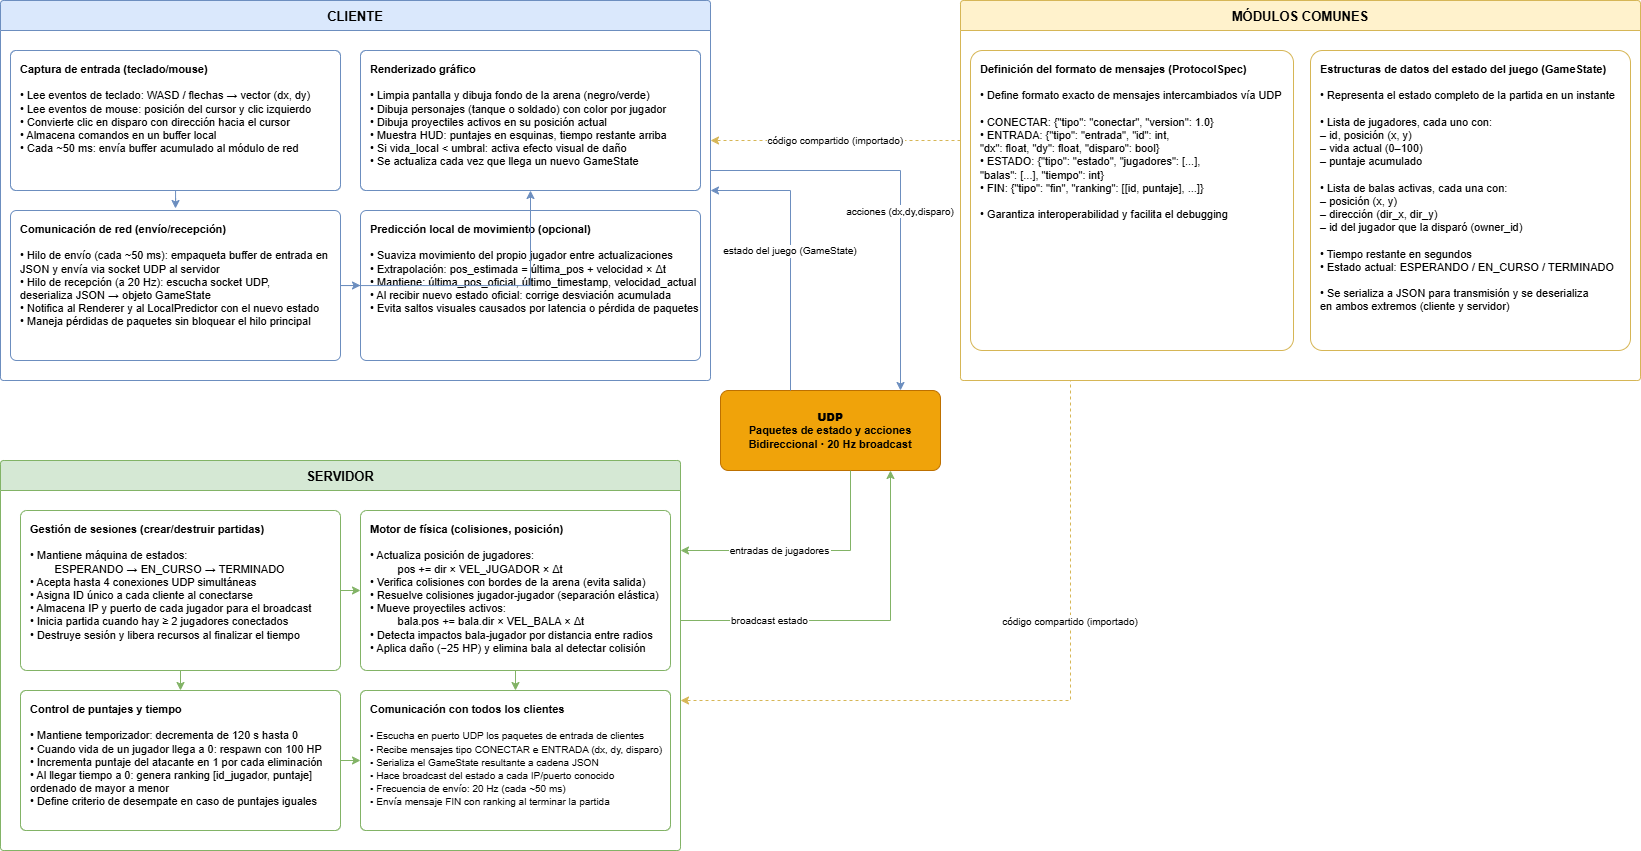
\includegraphics[width=0.95\columnwidth]{Imagenes/nivel2.png}
    \caption{Diagrama de Segundo Nivel.}
    \label{fig:nivel2}
\end{figure}

\subsection{Diagrama de Bloques --- Tercer Nivel}

El tercer nivel (Fig.~\ref{fig:nivel3}) expone los algoritmos internos y estructuras de datos de cada subm\'odulo.

\begin{figure}[!h]
    \centering
    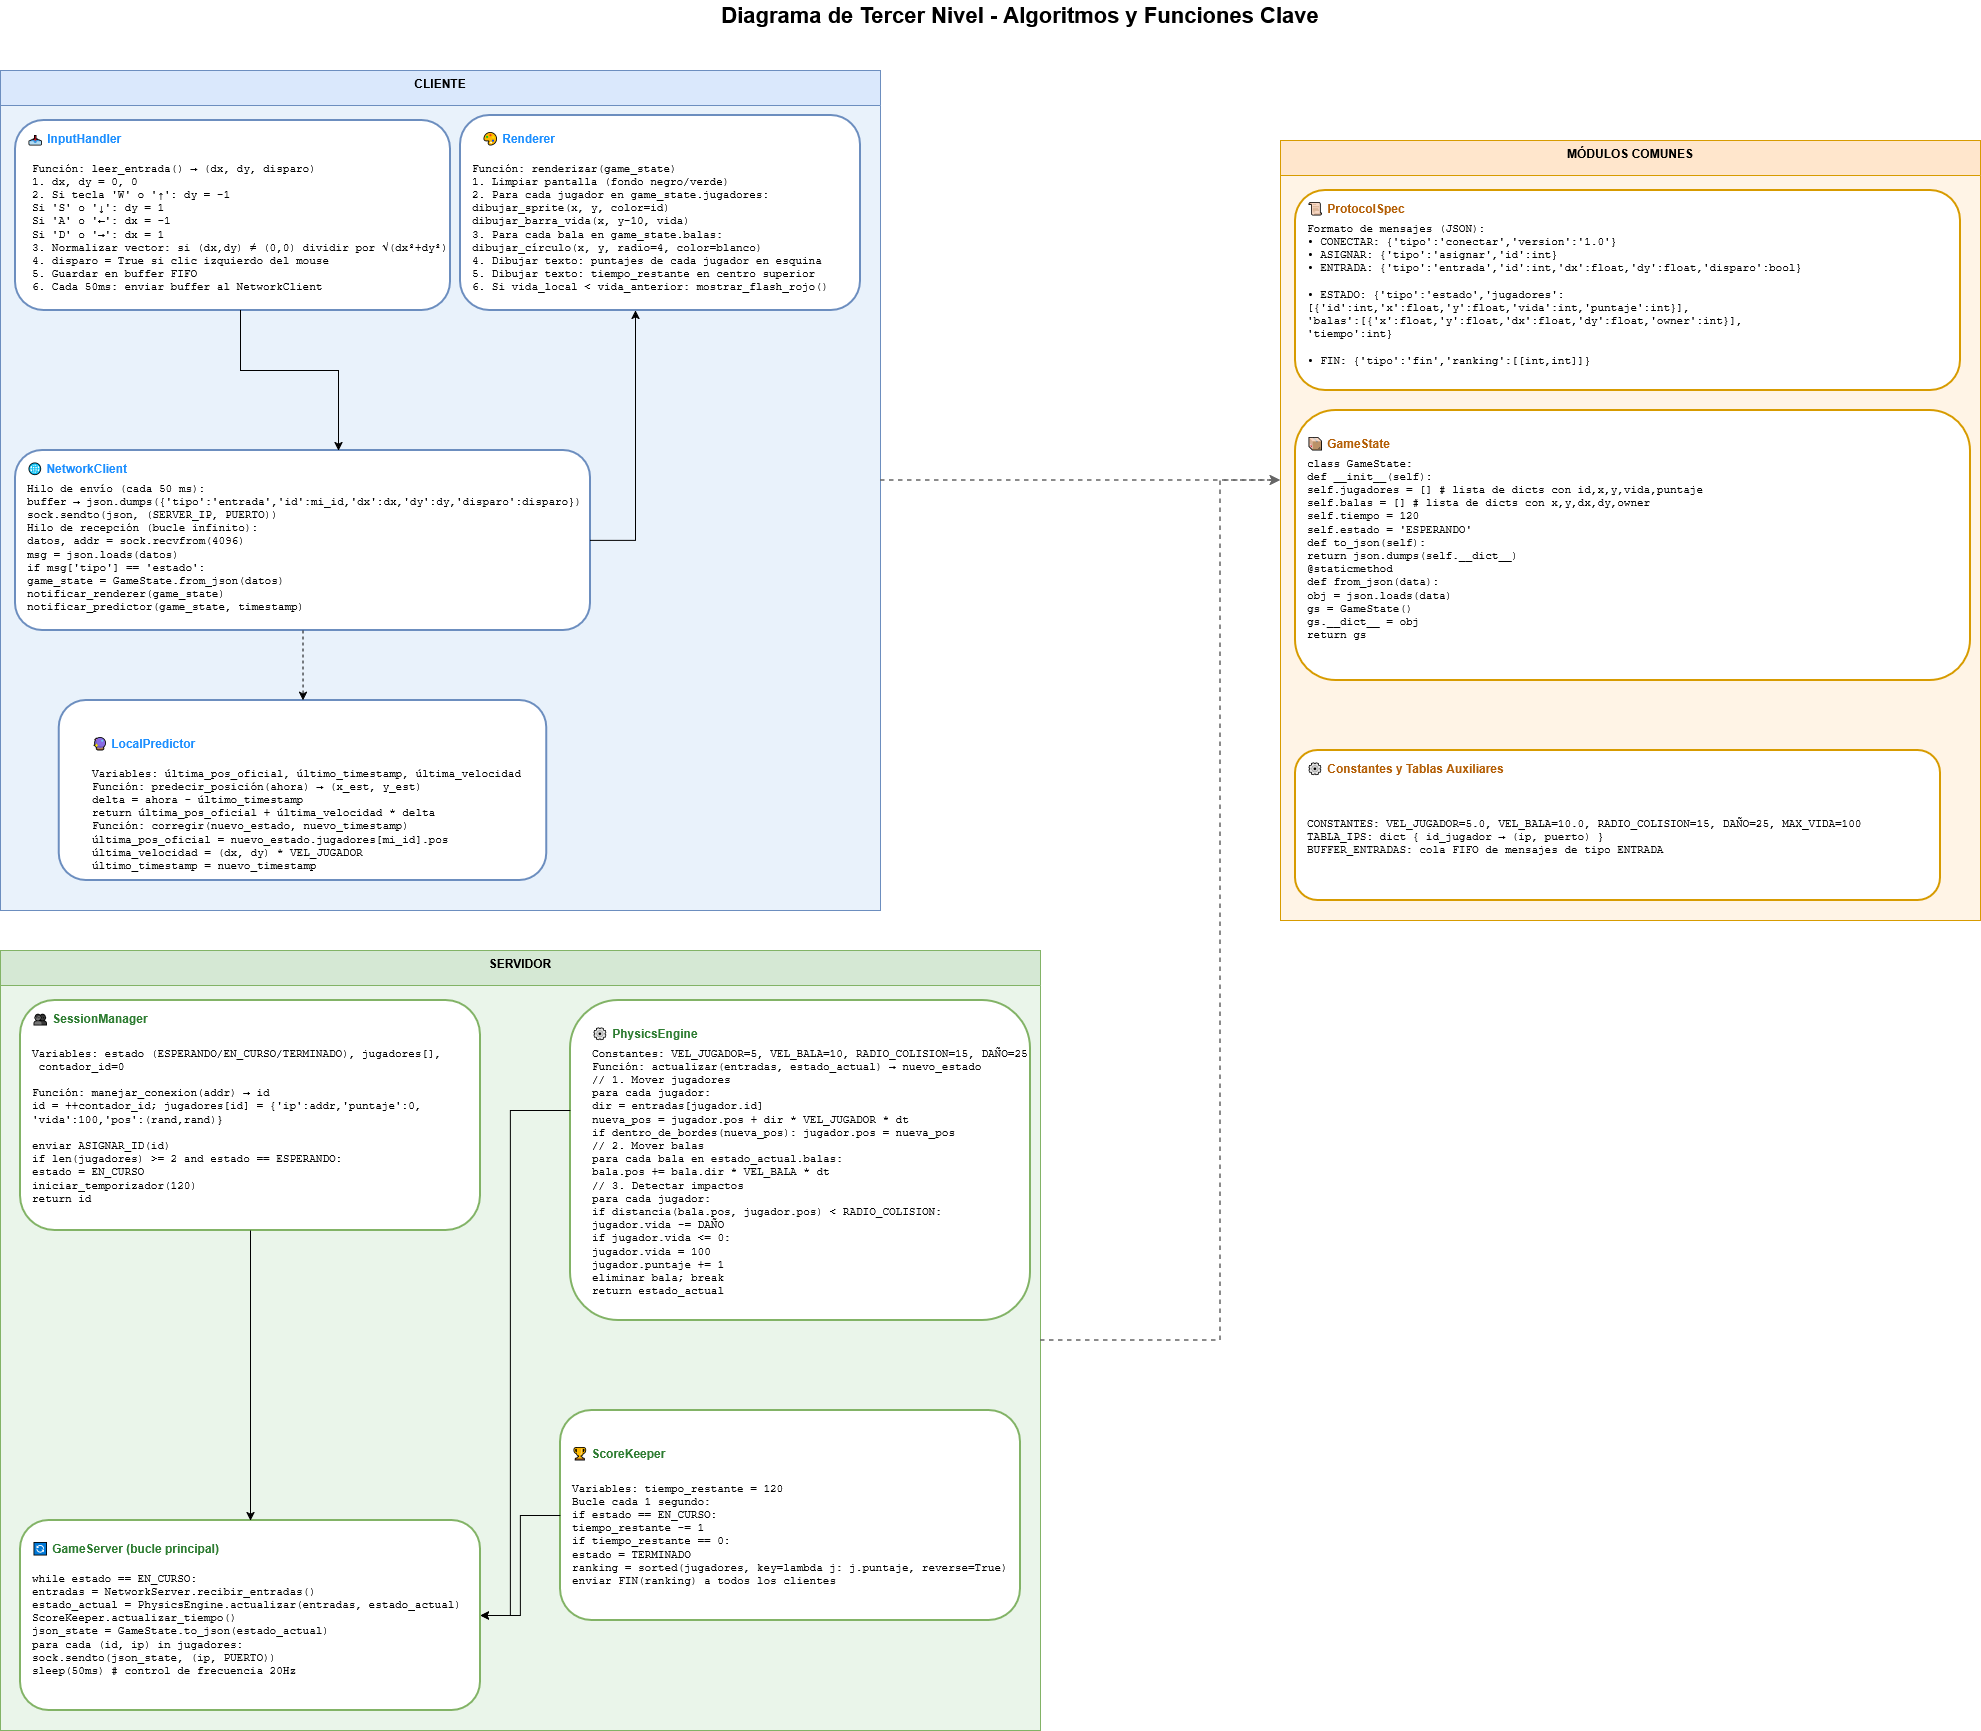
\includegraphics[width=0.95\columnwidth]{Imagenes/nivel3.png}
    \caption{Diagrama de Tercer Nivel.}
    \label{fig:nivel3}
\end{figure}

\subsection{Diagrama de Secuencia de Comunicaci\'on}

La Fig.~\ref{fig:secuencia} muestra el flujo de comunicaci\'on entre dos jugadores y el servidor, organizado en cuatro fases: conexi\'on y \textit{ready check}, cuenta regresiva, bucle de juego y finalizaci\'on.

\begin{figure}[!h]
    \centering
    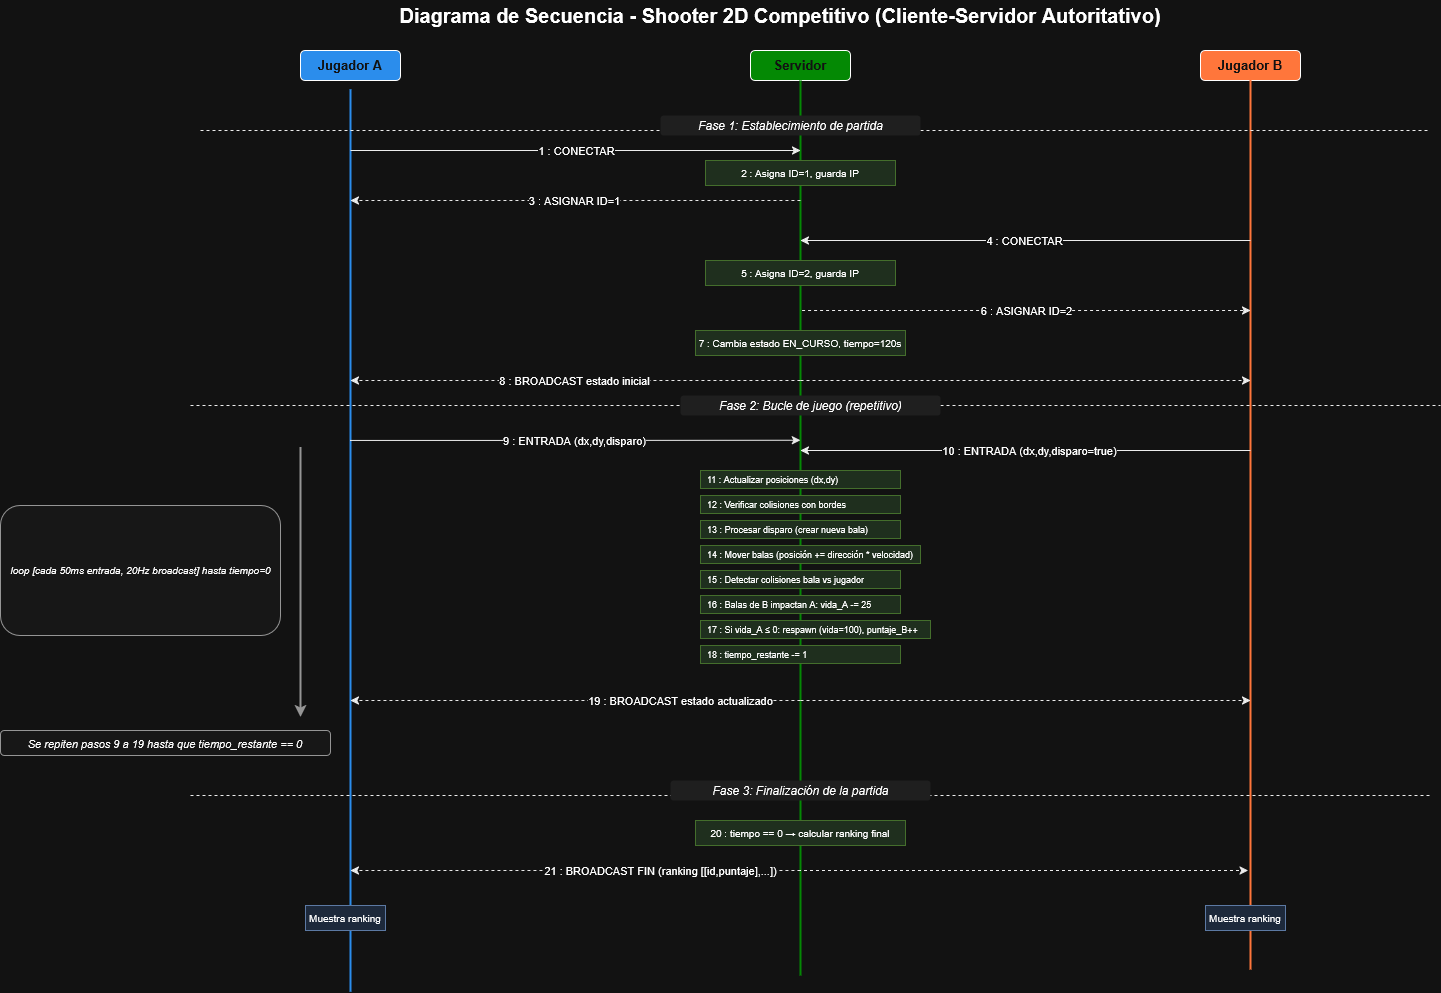
\includegraphics[width=0.95\columnwidth]{Imagenes/secuencia.png}
    \caption{Diagrama de Secuencia de Comunicaci\'on.}
    \label{fig:secuencia}
\end{figure}

%=============================================================
\section{Implementaci\'on}
%=============================================================

El sistema fue implementado en Python 3.13 con Pygame 2.x para el renderizado del cliente. El c\'odigo se organiza en tres archivos: \texttt{common.py} (m\'odulos compartidos, 158 l\'ineas), \texttt{server.py} (servidor autoritativo, 608 l\'ineas) y \texttt{client.py} (cliente con predicci\'on, 802 l\'ineas).

\subsection{Servidor Autoritativo (\texttt{server.py})}

\subsubsection{Estructuras de Datos}

El servidor utiliza tres \texttt{dataclass} para representar el estado del juego:

\begin{itemize}
    \item \textbf{Player}: \texttt{player\_id}, \texttt{address}, \texttt{name}, posici\'on $(x, y)$, \texttt{hp} (0--100), \texttt{score}, \texttt{deaths}, \texttt{damage\_dealt}, vector de apuntado (\texttt{aim\_x}, \texttt{aim\_y}), \texttt{next\_shot\_time}, estado de arma potenciada (\texttt{has\_power\_weapon}, \texttt{power\_weapon\_end}), detecci\'on de flanco ascendente (\texttt{was\_shooting}), estado de \textit{ready}.
    \item \textbf{Bullet}: \texttt{owner\_id}, posici\'on, velocidad $(v_x, v_y)$, tiempo de vida (\texttt{ttl} = 1.4~s).
    \item \textbf{Pickup}: \texttt{pickup\_id}, tipo (\texttt{weapon}/\texttt{health}), posici\'on, estado activo, tiempo de reaparici\'on.
\end{itemize}

\subsubsection{M\'aquina de Estados}

El servidor implementa una m\'aquina de estados con cinco fases:

\begin{enumerate}
    \item \textbf{waiting}: Acepta conexiones. Transiciona a \texttt{ready\_check} cuando hay $\geq 2$ jugadores.
    \item \textbf{ready\_check}: Espera a que todos los jugadores env\'ien el mensaje \texttt{ready}. Si un jugador se desconecta y quedan $< 2$, regresa a \texttt{waiting}.
    \item \textbf{countdown}: Cuenta regresiva de 3 segundos. Se difunde el valor restante a los clientes.
    \item \textbf{playing}: Bucle principal del juego. Termina cuando un jugador alcanza $\texttt{KILLS\_TO\_WIN} = 3$ eliminaciones o expira el temporizador de 120~s.
    \item \textbf{finished}: Muestra ranking durante 8 segundos. Luego regresa a \texttt{waiting} para una nueva ronda.
\end{enumerate}

\subsubsection{L\'ogica de Juego}

En cada iteraci\'on del bucle principal (60~Hz), el servidor ejecuta:

\begin{enumerate}
    \item Recepci\'on de todos los mensajes UDP pendientes.
    \item Remoci\'on de jugadores inactivos ($> 10$~s sin mensaje).
    \item Actualizaci\'on de la fase actual.
    \item Si est\'a en fase \texttt{playing}:
    \begin{enumerate}
        \item Actualizaci\'on de posiciones de jugadores seg\'un teclas recibidas.
        \item Resoluci\'on de colisiones jugador-obst\'aculo (\texttt{push\_circle\_from\_rect}).
        \item Procesamiento de disparos: semi-autom\'atico para arma base (flanco ascendente del clic), autom\'atico para arma potenciada.
        \item Movimiento de balas con detecci\'on de colisi\'on contra obst\'aculos, bordes y jugadores.
        \item Aplicaci\'on de da\~no (10\% del HP base por impacto). Si HP $\leq 0$: respawn en posici\'on aleatoria, incremento de score del atacante.
        \item Recolecci\'on de \textit{pickups}: arma potenciada (15~s de full-auto con cooldown 0.12~s) o restauraci\'on completa de HP.
        \item Separaci\'on el\'astica entre jugadores superpuestos.
    \end{enumerate}
    \item Broadcast del estado completo a todos los clientes a 20~Hz.
\end{enumerate}

\subsubsection{Pseudoc\'odigo del Motor de F\'isica}

El Algoritmo~\ref{alg:physics} muestra el pseudoc\'odigo del motor de f\'isica implementado.

\begin{algorithm}[htbp]
\caption{update\_game (servidor)}
\label{alg:physics}
\begin{algorithmic}[1]
\Require $dt$, $now$, $jugadores$, $balas$, $pickups$, $obst\acute{a}culos$
\For{$j$ en $jugadores$}
  \If{$j.power\_weapon$ y $now \geq j.power\_end$}
    \State $j.power\_weapon \gets \textbf{false}$
  \EndIf
  \State $j.pos \mathrel{+}= normalizar(j.teclas) \times VEL \times dt$
  \State $j.pos \gets clamp(j.pos,\ RADIO,\ ANCHO - RADIO)$
  \For{$obs$ en $obst\acute{a}culos$}
    \State $j.pos \gets empujar\_circulo(j.pos,\ RADIO,\ obs)$
  \EndFor
  \If{$j.power\_weapon$ \textbf{y} $j.disparo$ \textbf{y} $now \geq j.next\_shot$}
    \State $crear\_bala(j)$; $j.next\_shot \gets now + 0.12$
  \ElsIf{$j.disparo$ \textbf{y no} $j.was\_shoot$ \textbf{y} $now \geq j.next\_shot$}
    \State $crear\_bala(j)$; $j.next\_shot \gets now + 0.35$
  \EndIf
  \State $j.was\_shoot \gets j.disparo$
\EndFor
\For{$b$ en $balas$}
  \State $b.pos \mathrel{+}= b.vel \times dt$; $b.ttl \mathrel{-}= dt$
  \If{$b.ttl \leq 0$ \textbf{o} fuera\_limites($b$) \textbf{o} colision\_obs($b$)}
    \State eliminar $b$; \textbf{continuar}
  \EndIf
  \For{$j$ en $jugadores \setminus \{b.due\tilde{n}o\}$}
    \If{$dist(b, j) \leq RADIO\_B + RADIO\_J$}
      \State $j.hp \mathrel{-}= 10$; $b.due\tilde{n}o.da\tilde{n}o \mathrel{+}= 10$
      \If{$j.hp \leq 0$}
        \State $respawn(j)$; $b.due\tilde{n}o.score \mathrel{+}= 1$
      \EndIf
      \State eliminar $b$
    \EndIf
  \EndFor
\EndFor
\For{$p$ en $pickups$ activos}
  \For{$j$ en $jugadores$}
    \If{$dist(p, j) \leq RADIO\_P + RADIO\_J$}
      \State aplicar\_pickup($j$, $p$); desactivar($p$, $now$)
    \EndIf
  \EndFor
\EndFor
\State $separar\_jugadores\_superpuestos()$
\end{algorithmic}
\end{algorithm}

\subsection{Cliente (\texttt{client.py})}

\subsubsection{Arquitectura Multi-hilo}

El cliente utiliza tres hilos con acceso sincronizado mediante \texttt{threading.Lock}:

\begin{itemize}
    \item \textbf{Hilo principal}: Ejecuta el bucle de Pygame (eventos, captura de input, predicci\'on local, renderizado) a 60~FPS.
    \item \textbf{Hilo de env\'io} (\texttt{\_send\_loop}): Env\'ia el estado de teclas y posici\'on del mouse al servidor a 30~Hz. Utiliza \texttt{input\_lock} para leer las teclas de forma segura.
    \item \textbf{Hilo de recepci\'on} (\texttt{\_receive\_loop}): Escucha respuestas del servidor y actualiza el estado compartido. Utiliza \texttt{state\_lock} para escribir de forma segura.
\end{itemize}

\subsubsection{Predicci\'on Local (\texttt{LocalPredictor})}

La clase \texttt{LocalPredictor} implementa predicci\'on del lado del cliente con reconciliaci\'on por \textit{lerp}:

\begin{enumerate}
    \item \textbf{apply\_input}: Cada \textit{frame}, aplica $pos += normalizar(teclas) \times VELOCIDAD \times dt$ y resuelve colisiones con obst\'aculos localmente.
    \item \textbf{correct}: Cuando llega un estado del servidor, corrige la posici\'on predicha:
    \begin{equation}
    pos_{pred} \mathrel{+}= (pos_{servidor} - pos_{pred}) \times 0.3
    \end{equation}
    El factor 0.3 suaviza la correcci\'on en $\sim$3--4 \textit{frames}, evitando saltos bruscos~\cite{gambetta2018}.
\end{enumerate}

\subsubsection{Renderizado}

El cliente implementa un \textit{pipeline} de renderizado por capas:

\begin{enumerate}
    \item \textbf{Fondo pre-renderizado}: Mapa militar generado una sola vez con semilla determin\'istica (bandas de pasto, parches de tierra, ret\'icula t\'actica, marcadores de spawn, muros perimetrales).
    \item \textbf{Obst\'aculos}: Bloques de concreto con efecto 3D (resaltado superior izquierdo, sombra inferior derecha, l\'inea central de detalle).
    \item \textbf{Pickups}: Estrella dorada para arma potenciada, c\'irculo blanco con cruz roja para salud.
    \item \textbf{Balas}: C\'irculos naranjas con borde y n\'ucleo claro.
    \item \textbf{Tanques}: Cuerpo del casco con pistas y secciones de oruga, torreta circular, ca\~n\'on, barra de HP, etiqueta de ID. Todo rotado seg\'un el \'angulo de apuntado. Soporte opcional para sprites personalizados.
    \item \textbf{HUD}: Panel superior con temporizador, tarjetas de jugador (color, nombre, kills, barra de HP, indicador de arma), estado de fase y objetivo.
    \item \textbf{Overlays}: Cuenta regresiva centrada durante fase \texttt{countdown}; panel de ranking con columnas (Jugador, Kills, Muertes, Da\~no) durante fase \texttt{finished}.
\end{enumerate}

\subsubsection{Sistema de Audio}

El cliente carga archivos WAV desde \texttt{assets/sounds/} con \textit{fallback} silencioso si no existen:
\begin{itemize}
    \item \texttt{shoot}: Al presionar clic izquierdo (flanco ascendente) durante fase \texttt{playing}.
    \item \texttt{hit}: Cuando el HP del jugador local disminuye.
    \item \texttt{kill}: Cuando el jugador local muere y reaparece.
    \item \texttt{game\_over}: Al transicionar a fase \texttt{finished}.
\end{itemize}

\subsection{M\'odulo Com\'un (\texttt{common.py})}

\subsubsection{Constantes del Protocolo}

\begin{table}[!h]
\centering
\caption{Par\'ametros principales del sistema.}
\label{tab:params}
\begin{tabular}{@{}ll@{}}
\toprule
\textbf{Par\'ametro} & \textbf{Valor} \\
\midrule
\'Area de juego & 960 $\times$ 540 px \\
M\'ax. jugadores & 4 \\
Velocidad jugador & 220 px/s \\
Velocidad bala & 520 px/s \\
HP & 100 (da\~no base: 10) \\
Cooldown arma base & 0.35 s (semi-auto) \\
Cooldown arma potenciada & 0.12 s (full-auto, 15 s) \\
Tick servidor & 60 Hz \\
Broadcast & 20 Hz \\
Input cliente & 30 Hz \\
Condici\'on de victoria & 3 kills o 120 s \\
Pickups respawn & 10 s \\
\bottomrule
\end{tabular}
\end{table}

\subsubsection{Generaci\'on de Obst\'aculos}

Los obst\'aculos se generan determin\'isticamente con \texttt{random.Random(seed=42)}: 6 rect\'angulos en la zona central del mapa ($x \in [180, 780]$, $y \in [150, 390]$), con zona de exclusi\'on de 70~px alrededor de los puntos de spawn y separaci\'on m\'inima de 15~px entre obst\'aculos.

\subsubsection{Funciones de Colisi\'on}

\begin{itemize}
    \item \texttt{circle\_rect\_overlap(cx, cy, r, rx, ry, rw, rh)}: Retorna \texttt{True} si un c\'irculo colisiona con un rect\'angulo alineado a ejes. Utiliza la t\'ecnica de punto m\'as cercano.
    \item \texttt{push\_circle\_from\_rect(...)}: Empuja el c\'irculo fuera del rect\'angulo. Maneja el caso especial donde el centro del c\'irculo est\'a dentro del rect\'angulo (empuja por el borde m\'as cercano).
\end{itemize}

\subsection{Protocolo de Comunicaci\'on}

Los mensajes se serializan como JSON compacto (\texttt{separators=(",", ":")}) y se codifican en UTF-8. Los tipos de mensaje implementados son:

\begin{lstlisting}[caption={Mensajes del protocolo.},label={lst:protocol2}]
// Cliente -> Servidor
{"type":"connect","name":"Jugador 1"}
{"type":"input","id":1,"keys":{"up":true,...},
 "aim":[480,270]}
{"type":"ready"}
{"type":"disconnect","id":1}

// Servidor -> Cliente
{"type":"welcome","id":1}
{"type":"full","reason":"..."}
{"type":"state","phase":"playing",
 "time_left":95,"winner_id":null,
 "ranking":[],"ready_count":2,
 "total_players":2,"countdown":0,
 "players":[{"id":1,"name":"J1",
  "x":80,"y":80,"hp":100,"score":0,
  "aim":[1,0],"pw":false,"ready":true}],
 "bullets":[{"owner_id":1,"x":120,"y":80}],
 "pickups":[{"id":1,"type":"weapon",
  "x":400,"y":300}]}
\end{lstlisting}

%=============================================================
\section{Pruebas de Implementaci\'on}
%=============================================================

Se verificaron todas las funcionalidades especificadas en el documento de dise\~no. La Tabla~\ref{tab:tests} resume las pruebas realizadas.

\begin{table}[!h]
\centering
\caption{Verificaci\'on de funcionalidades implementadas.}
\label{tab:tests}
\begin{tabular}{@{}p{5.2cm}c@{}}
\toprule
\textbf{Funcionalidad} & \textbf{Estado} \\
\midrule
Conexi\'on UDP cliente-servidor & \checkmark \\
Hasta 4 jugadores simult\'aneos & \checkmark \\
Movimiento WASD / flechas & \checkmark \\
Apuntado con mouse & \checkmark \\
Disparo semi-autom\'atico (arma base) & \checkmark \\
Disparo autom\'atico (arma potenciada) & \checkmark \\
Detecci\'on colisi\'on bala-jugador & \checkmark \\
Detecci\'on colisi\'on bala-obst\'aculo & \checkmark \\
Colisi\'on jugador-obst\'aculo (push-out) & \checkmark \\
Colisi\'on jugador-jugador (separaci\'on) & \checkmark \\
Colisi\'on jugador-bordes (clamping) & \checkmark \\
Sistema de HP (da\~no 10\%, respawn) & \checkmark \\
Sistema de kills y puntaje & \checkmark \\
Pickup: arma potenciada (15~s) & \checkmark \\
Pickup: restauraci\'on de HP & \checkmark \\
Respawn de pickups (10~s) & \checkmark \\
Predicci\'on local de movimiento & \checkmark \\
Reconciliaci\'on con lerp (0.3) & \checkmark \\
Multi-hilo (send, receive, render) & \checkmark \\
Thread-safety con locks & \checkmark \\
Sistema de fases (5 estados) & \checkmark \\
Ready check + countdown & \checkmark \\
Victoria por kills (3) o tiempo (120~s) & \checkmark \\
Ranking final (kills, muertes, da\~no) & \checkmark \\
HUD con timer, HP, kills & \checkmark \\
Efectos de sonido (4 tipos) & \checkmark \\
Mapa militar pre-renderizado & \checkmark \\
Tanques con rotaci\'on por aim & \checkmark \\
Broadcast de estado a 20~Hz & \checkmark \\
Desconexi\'on por inactividad (10~s) & \checkmark \\
\bottomrule
\end{tabular}
\end{table}

\subsection{Procedimiento de Pruebas}

Para verificar el funcionamiento multijugador:

\begin{enumerate}
    \item Se inicia el servidor: \texttt{python server.py [puerto]}
    \item Se inician 2--4 clientes: \texttt{python client.py <IP> <puerto> <nombre>}
    \item Para LAN: se utiliza la IP local del servidor (e.g., \texttt{192.168.1.X}).
    \item Para VPN: se instala ZeroTier en ambos equipos, se unen a la misma red virtual, y se utiliza la IP asignada por ZeroTier.
    \item Cada jugador presiona el bot\'on ``EMPEZAR'' en la interfaz.
    \item Tras la cuenta regresiva de 3 segundos, comienza la partida.
    \item Se verifica movimiento, disparo, colisiones, pickups y puntaje.
    \item La partida termina al alcanzar 3 kills o agotar 120~s, mostrando el ranking.
\end{enumerate}

%=============================================================
\begin{thebibliography}{00}

\bibitem{tanenbaum2011}
A.~S. Tanenbaum and D.~J. Wetherall,
\textit{Computer Networks}, 5th~ed.
Upper Saddle River, NJ: Pearson Prentice Hall, 2011.

\bibitem{kurose2017}
J.~F. Kurose and K.~W. Ross,
\textit{Computer Networking: A Top-Down Approach}, 7th~ed.
Hoboken, NJ: Pearson, 2017.

\bibitem{forouzan2012}
B.~A. Forouzan,
\textit{Data Communications and Networking}, 5th~ed.
New York, NY: McGraw-Hill, 2012.

\bibitem{rfc768}
J.~Postel,
``User Datagram Protocol,''
IETF RFC 768, Aug. 1980.

\bibitem{pressman2014}
R.~S. Pressman and B.~R. Maxim,
\textit{Software Engineering: A Practitioner's Approach}, 8th~ed.
New York, NY: McGraw-Hill Education, 2014.

\bibitem{gambetta2018}
G.~Gambetta,
``Fast-Paced Multiplayer: Client-Server Game Architecture,''
\textit{Gabriel Gambetta's Blog}, 2018.

\bibitem{pygame2023}
Pygame Community,
\textit{Pygame Documentation}, version 2.x.
2023.

\end{thebibliography}

\end{document}
